\section{Testing und Laufzeitanalyse}
\label{sec:testing_und_laufzeitanalyse}

\subsection{Testing}
\label{ssec:testing}

\subsubsection{Teststrategie}
\label{sssec:teststrategie}

% Beschreibung der Teststrategie
Die Testfälle wurden nach der Methode $\ldots$ ausgewählt.
Die Testfälle sind in Tabelle \ref{tab:example_testcases} aufgelistet.\footnote{Die Testfälle sind im Anhang \ref{sec:anhang} zu finden.}

\begin{figure}[H]
    \centering
    % unterteilt nach Normalfällen, Grenzfällen, Fehlerfällen
    \begin{tabular}{|l|l|l|l|}
        \hline
        \textbf{Testfall}    & \textbf{Eingabe} & \textbf{Erwartete Ausgabe} & \textbf{Bemerkung} \\
        \hline
        \hline
        \textbf{Normalfälle} &                  &                            &                    \\
        \hline
        \hline
        \textbf{Grenzfälle}  &                  &                            &                    \\
        \hline
        \hline
        \textbf{Fehlerfälle} &                  &                            &                    \\
        \hline
    \end{tabular}
    \caption{Beispiel für eine Tabelle mit Testfällen}
    \label{tab:example_testcases}
\end{figure}

\subsubsection{Beobachtungen}
\label{sssec:beobachtungen}

% Beschreibung der Beobachtungen
Es wurden folgende Beobachtungen gemacht:
\begin{itemize}
    \item $\ldots$
    \item $\ldots$
    \item $\ldots$
\end{itemize}

\subsection{Laufzeitanalyse}
\label{ssec:laufzeitanalyse}

% Beschreibung der Laufzeitanalyse
Die Laufzeitanalyse wurde mit $\ldots$ durchgeführt.
Jeder Testfall wurde $\ldots$ mal ausgeführt und im Anschluss die Laufzeiten gemittelt.

Für die einzelnen Testfälle aus Tabelle \ref{tab:example_testcases} ergeben sich die Laufzeiten in Tabelle \ref{tab:example_runtime}.

\begin{figure}[H]
    \centering
    % unterteilt nach Normalfällen, Grenzfällen, Fehlerfällen
    % median, mean, standard deviation
    \begin{tabular}{|l|l|l|l|}
        \hline
        \textbf{Testfall}    & \textbf{Median} & \textbf{Mittelwert} & \textbf{Standardabweichung} \\
        \hline
        \hline
        \textbf{Normalfälle} &                 &                     &                             \\
        \hline
        \hline
        \textbf{Grenzfälle}  &                 &                     &                             \\
        \hline
        \hline
        \textbf{Fehlerfälle} &                 &                     &                             \\
        \hline
    \end{tabular}
    \caption{Beispiel für eine Tabelle mit Laufzeiten}
    \label{tab:example_runtime}
\end{figure}

% graphische Darstellung der Laufzeiten
\begin{figure}[H]
    \centering
    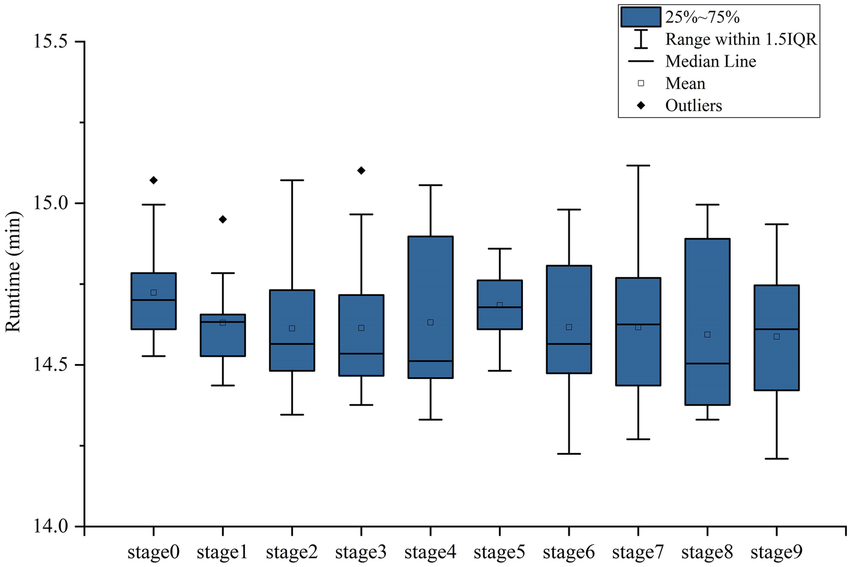
\includegraphics[width=0.8\textwidth]{figures/example_runtime.png}
    \caption{Beispiel für eine graphische Darstellung der Laufzeiten}
    \label{fig:example_runtime}
\end{figure}

Besonders auffällig ist $\ldots$, da der Algorithmus in $\mathcal{O}(n^m)$ läuft.

Für den praktischen Einsatz muss die Laufzeit nochmals verbessert werden.
Siehe dazu Abschnitt \ref{ssec:ausblick}.